\section{Konstrukce dvířek}\label{sec:konstrukce-dvirek}
Elektricky ovládaná dvířka systému Coopmaster plní hlavní požadavek, který na systém babička měla.
Slouží k automatickému a bezpečnému otevírání vstupu do kurníku.

Aktuální verze dvířek je sestavena ze standardních hliníkových profilů a spojovací komponent.
Pro pohyb dvířek se pro tento prototyp jeví jako nejsnažší volba táhlový motor.
Pracuje na napětí 12V stejnosměrných (popis v sekci~\ref{sec:tahlovy-motor}).
Je vybaven nastavitelnými dorazy, které umožují zastavit rozmezí ve kterém se má výsuv pohybovat.
Tělo motoru je připevněno k rámu dveří.
Technický výkres motoru jsem připojil. ~\ref{fig:instalace_dvere_tahlovy_motor}
Pohyblivá část je volně připojena k vertikálně se pohybujícímu kovovému plátu, který slouží jako spouštěcí dveře.

První návrh počítal s pevným připojením mezi dveřmi a motorem, ale během testů se ukázalo, jak důležité je motor propojit s dvířky nějakým flexibilním spojem.
Pokud by byl totiž plát připevněn pevně k motoru, mohla by se snadno stát z dvířek gilotina.
Táhlový motor je schopen totiž vyvinout sílu až 200 kg (2000 N).

\begin{figure}[h]
    \centering
    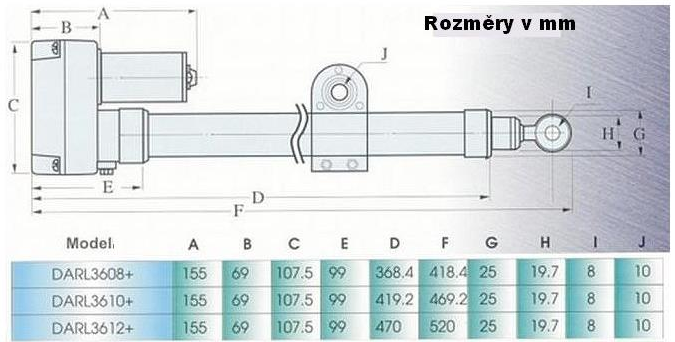
\includegraphics[width=\textwidth]{img/instalace_dvere_tahlovy_motor}
    \caption{Rozmery tahloveho motoru}
    \label{fig:instalace_dvere_tahlovy_motor}
\end{figure}

Pokud by z nějakého důvodu zůstalo cokoliv v průchodu mohlo by dojít bude ke zranění slepice nebo poškození dveřního mechanizmu.
Já jsem ve svém řešení použil silonový provázek.

Musel jsem se vypořádat s faktem, že motor má nedostatečný výsuv.
Řešením byla instalace kladky, která zdvojnásobila zdvih dveří tak , aby slepice vůbec prolezla pod plátem.

Ačkoli má toto řešení řadu nevýhod, tak bylo realizováno jednoduše z toho důvodu, že jsem většinu součástek měl doma již z minulých projektů.

I kdyby se do budoucna vyřešily zmíňované problémy, řešení by pořád nebylo produkční, protože hliníkové součásti společně s motorem jsou příliš drahé.
Z ekonomického hlediska je jasné, že by si malý chovateln nechtěl do kurníku instalovat dvířka, která svou cenou převýší cenu vajec, které vyprodukujete za rok.

Nicméně projekt je aktuálně ve fázi vývoje, kdy řeším spíše softwarovou než hardwarovou stránku.
Pro testovací účely je mechanismus aktuálních dvířek vyhovující.
Vyhodou hlinikových profilu je možnost snadných úprav a ladění konstukce.

Na obrázku~\ref{fig:proto_dvirka} můžete vidět aktuální podobu dvířek instalovaných u kurníku.

\begin{figure}[h]
    \centering
    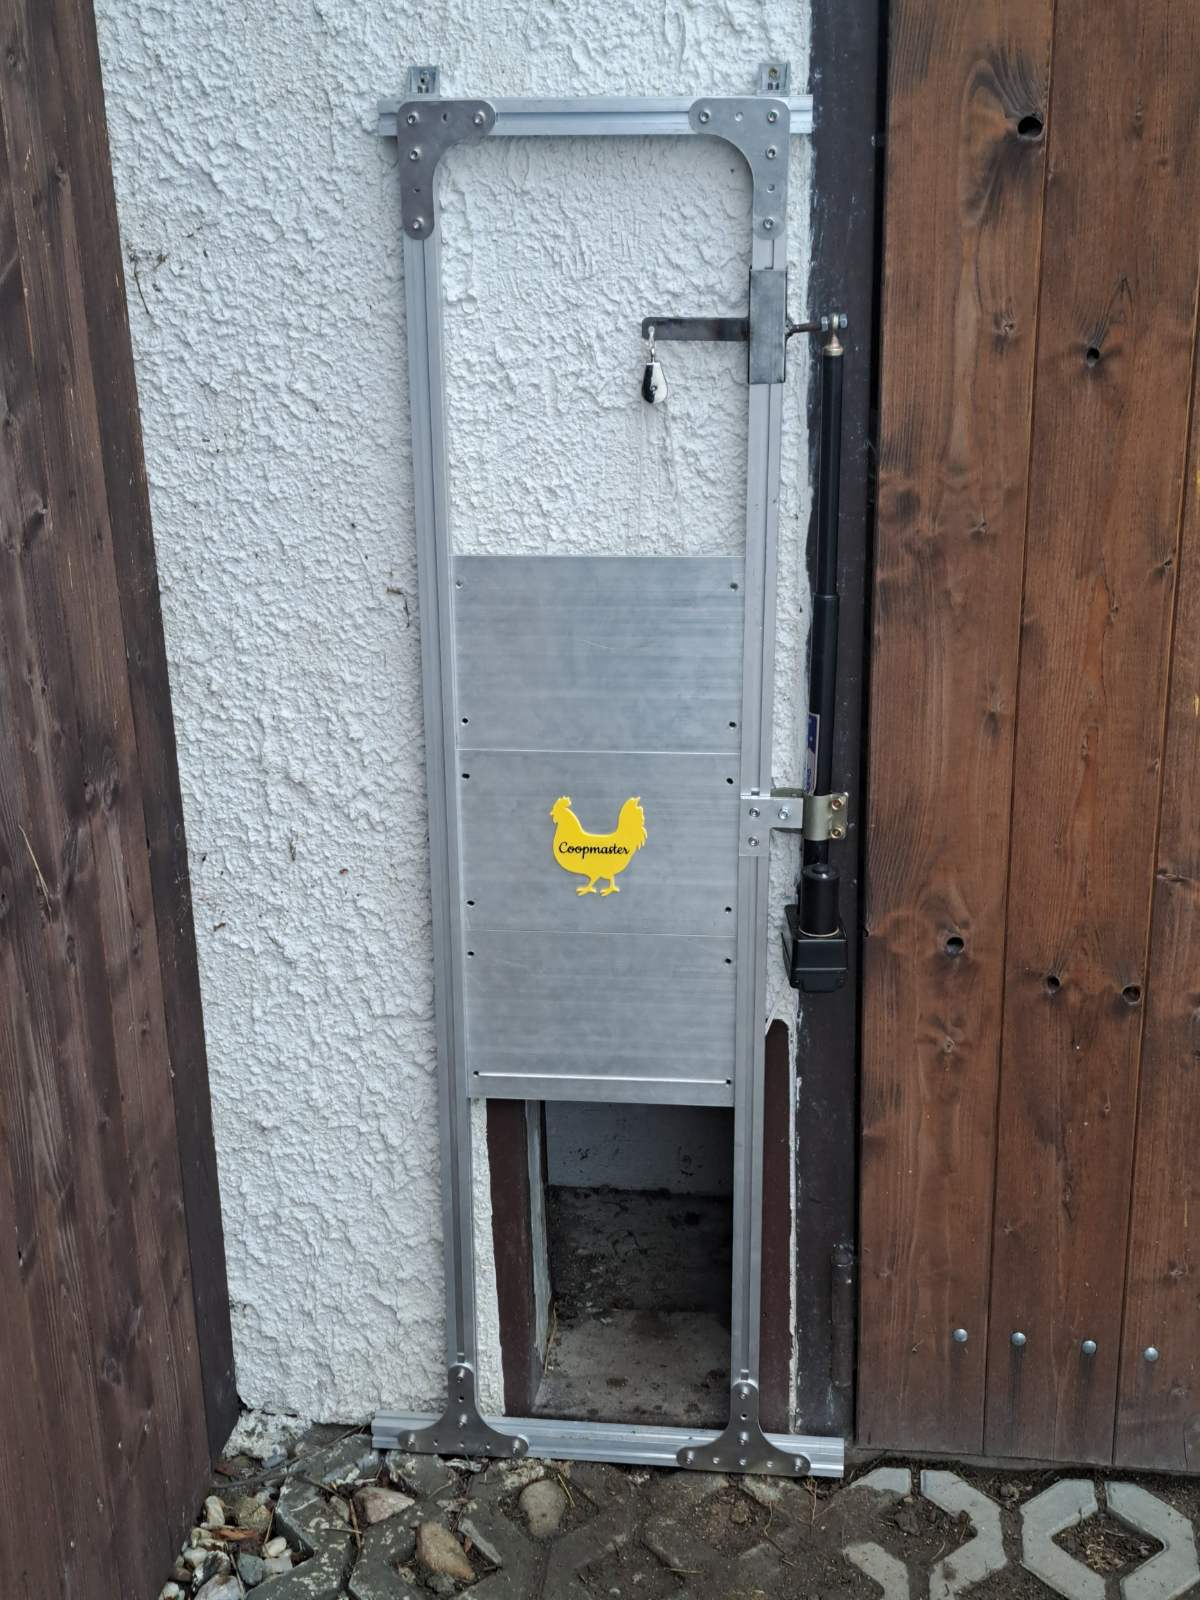
\includegraphics[width=\textwidth]{img/proto_dvirka}
    \caption{Instalovaný prototyp dvířek}
    \label{fig:proto_dvirka}
\end{figure}

Myslím, si že pro finální instalaci budu muset zvážit úpravy konstrukce a pohonu.
Hlinková konstrukce ze stavebnicového systému je drahá a věřím, že i samotný pohon půjde realizovat levněji.




